\section{GUI Class Reference}
\label{classGUI}\index{GUI@{GUI}}
Inheritance diagram for GUI:\begin{figure}[H]
\begin{center}
\leavevmode
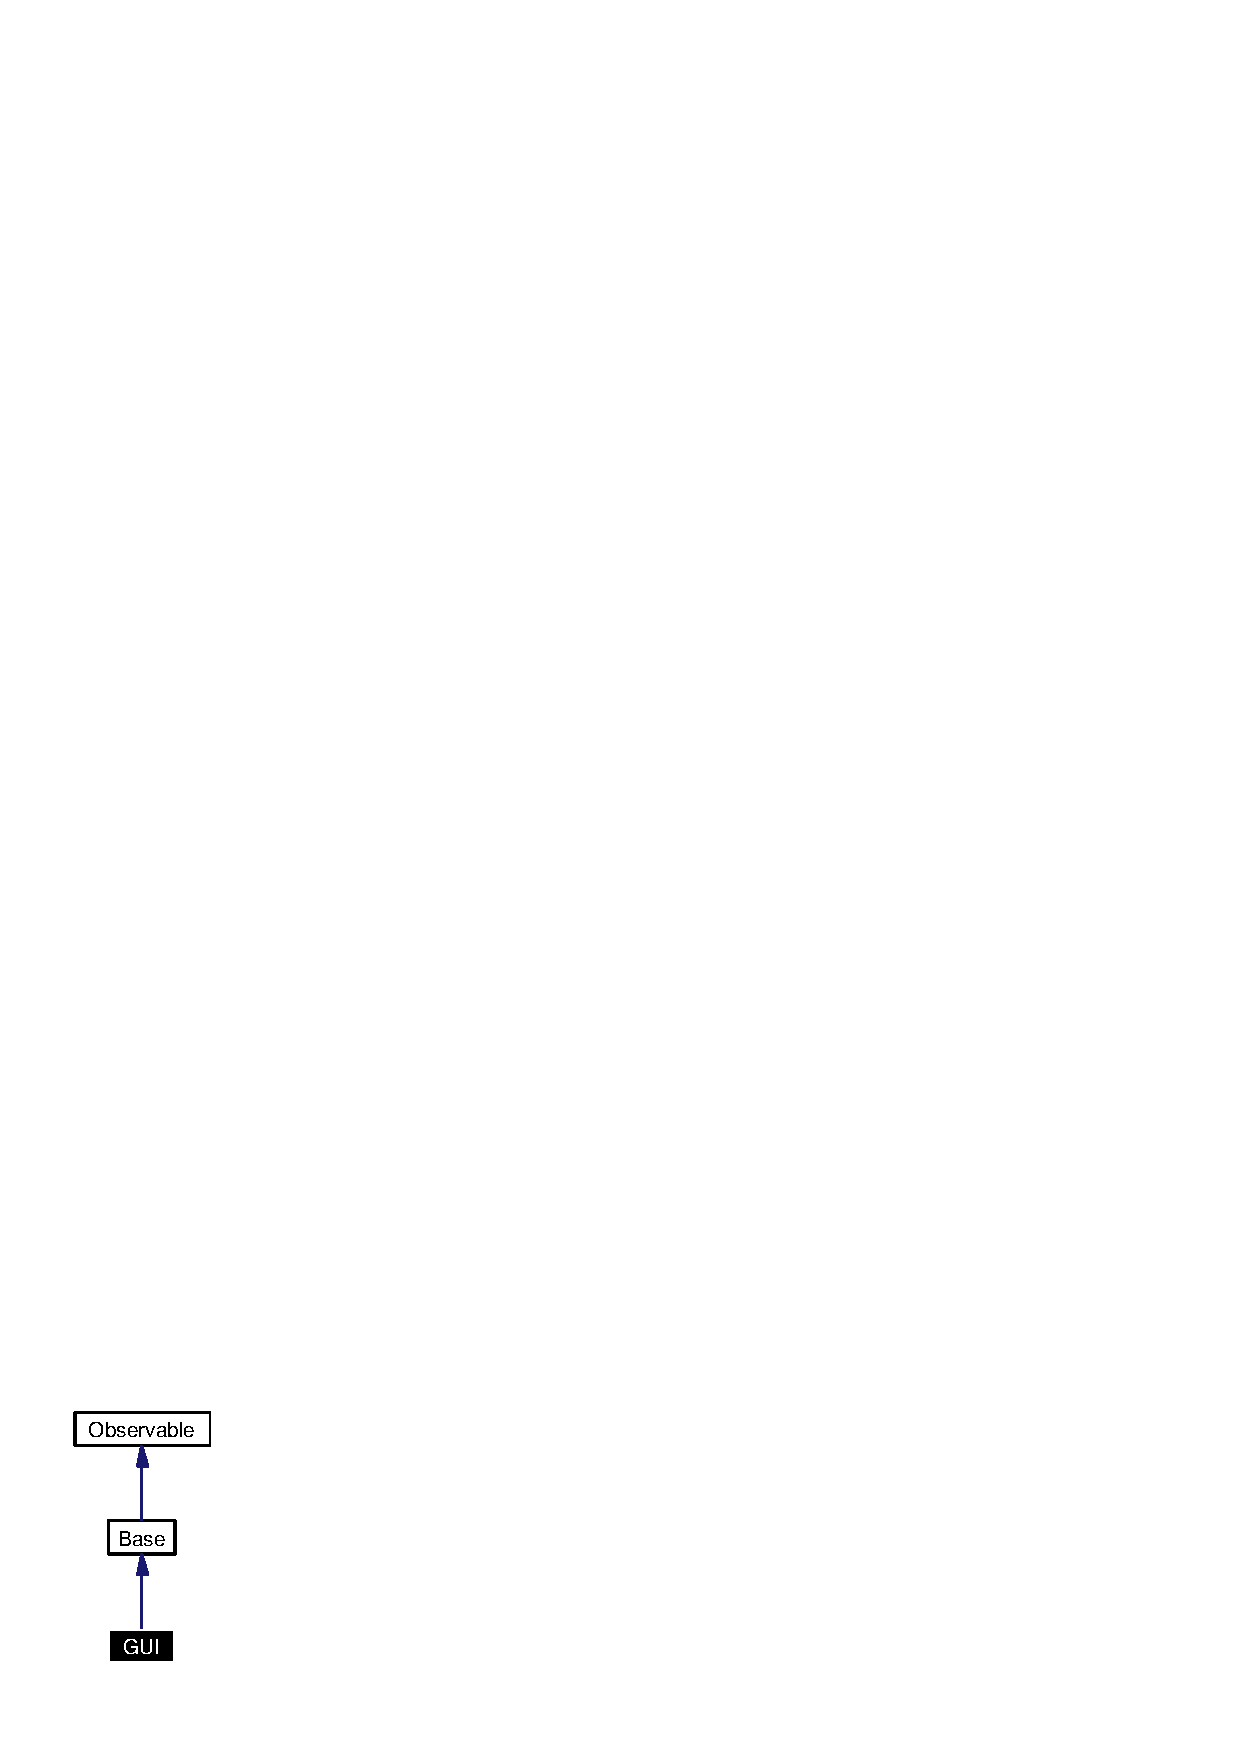
\includegraphics[width=50pt]{classGUI__inherit__graph}
\end{center}
\end{figure}
Collaboration diagram for GUI:\begin{figure}[H]
\begin{center}
\leavevmode
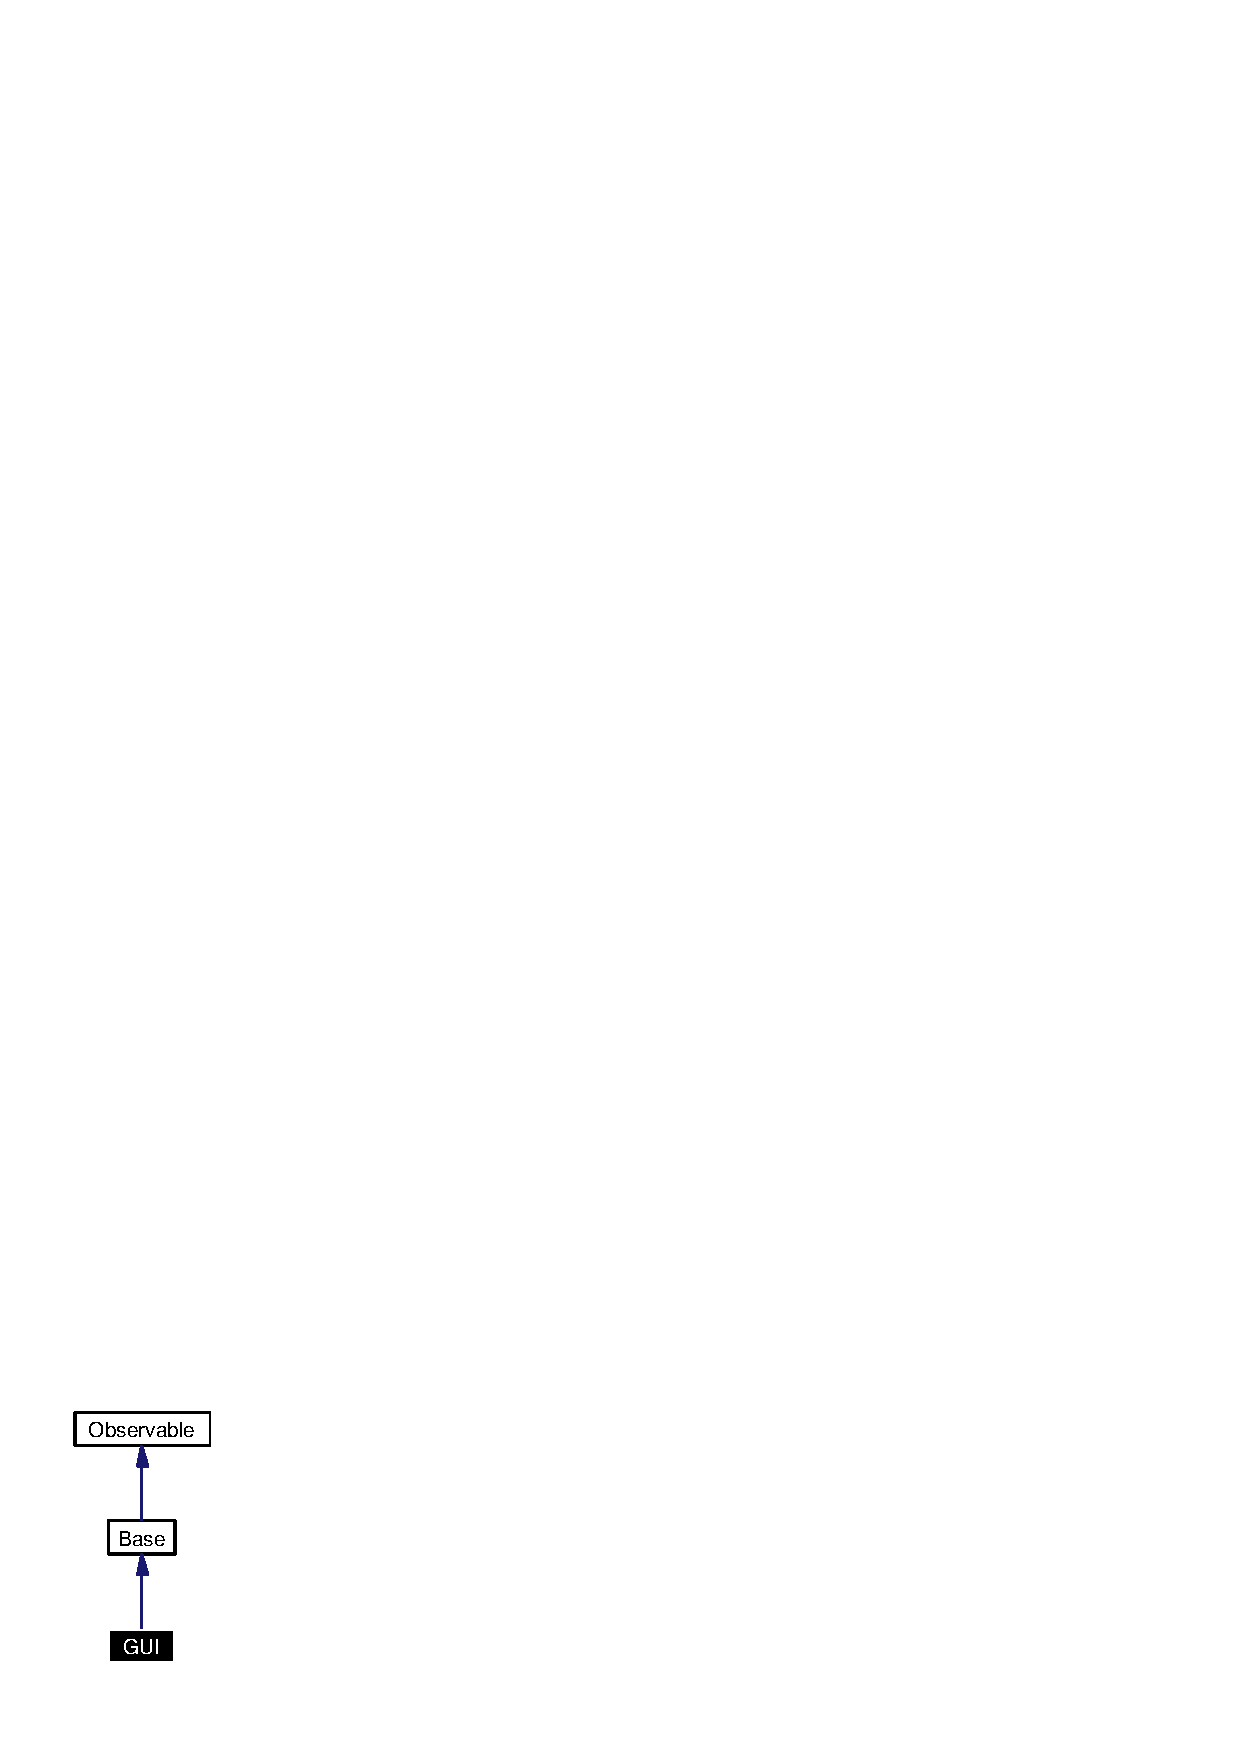
\includegraphics[width=50pt]{classGUI__coll__graph}
\end{center}
\end{figure}
\subsection*{Public Member Functions}
\begin{CompactItemize}
\item 
{\bf gui\_\-list\_\-user\_\-processes} (\$user, \$offset, \$max\-Records, \$sort\_\-mode, \$find, \$where='')
\item 
{\bf gui\_\-list\_\-user\_\-activities} (\$user, \$offset, \$max\-Records, \$sort\_\-mode, \$find, \$where='')\label{classGUI_a1}

\item 
{\bf gui\_\-list\_\-user\_\-instances} (\$user, \$offset, \$max\-Records, \$sort\_\-mode, \$find, \$where='')\label{classGUI_a2}

\item 
{\bf gui\_\-abort\_\-instance} (\$user, \$activity\-Id, \$instance\-Id)\label{classGUI_a3}

\item 
{\bf gui\_\-exception\_\-instance} (\$user, \$activity\-Id, \$instance\-Id)\label{classGUI_a4}

\item 
{\bf gui\_\-send\_\-instance} (\$user, \$activity\-Id, \$instance\-Id)\label{classGUI_a5}

\item 
{\bf gui\_\-release\_\-instance} (\$user, \$activity\-Id, \$instance\-Id)\label{classGUI_a6}

\item 
{\bf gui\_\-grab\_\-instance} (\$user, \$activity\-Id, \$instance\-Id)\label{classGUI_a7}

\end{CompactItemize}


\subsection{Detailed Description}
This class provides methods for use in typical user interface scripts 



Definition at line 8 of file GUI.php.

\subsection{Member Function Documentation}
\index{GUI@{GUI}!gui_list_user_processes@{gui\_\-list\_\-user\_\-processes}}
\index{gui_list_user_processes@{gui\_\-list\_\-user\_\-processes}!GUI@{GUI}}
\subsubsection{\setlength{\rightskip}{0pt plus 5cm}GUI::gui\_\-list\_\-user\_\-processes (\$ {\em user}, \$ {\em offset}, \$ {\em max\-Records}, \$ {\em sort\_\-mode}, \$ {\em find}, \$ {\em where} = '')}\label{classGUI_a0}


List user processes, user processes should follow one of these conditions: 1) The process has an instance assigned to the user 2) The process has a begin activity with a role compatible to the user roles 3) The process has an instance assigned to '$\ast$' and the roles for the activity match the roles assigned to the user The method returns the list of processes that match this and it also returns the number of instances that are in the process matching the conditions. 

Definition at line 22 of file GUI.php.

The documentation for this class was generated from the following file:\begin{CompactItemize}
\item 
GUI.php\end{CompactItemize}
